\chapter{Casi di Studio}
\label{cap:esempi}

\section{Introduzione}
Nel capitolo \ref{cap:tc} è stato dimostrato il funzionamento del traffic shaping con il comando \texttt{tc}, citando anche i limiti che gli appartengono.
Invece, in questo capitolo, si vuole dimostrare la fattibilità del traffic shaping tramite l'utilizzo di Kathará e Damper, elencando eventuali limiti presenti. \\ 
Saranno tre diversi scenari, ognuno utile a capire i diversi aspetti della strategia di shaping in userspace. \\
\vspace*{0.01\textheight}
Per usare correttamente Damper tramite Kathará, ho creato un immagine Docker, 
al cui interno ho compilato il programma come visto nel capitolo \ref{cap:userspace}
e aggiunto un file \texttt{damper.conf} come base in \texttt{/etc/damper/}.

\begin{docker}[Dockerfile personalizzato]
# Usata la stessa immagine di base per compilare
FROM kathara/core:latest AS damper
RUN apt update && apt install -y --no-install-recommends \
    libnetfilter-queue-dev \
    gcc \
    build-essential && \
    apt clean && rm -rf /tmp/* /var/lib/apt/lists/* /var/tmp/*
WORKDIR /src
RUN git clone --depth 1 https://github.com/vmxdev/damper.git .
RUN gcc -Wall -pedantic damper.c modules.conf.c -o damper -lnetfilter_queue -pthread -lrt -lm

# Immagine kathara/base
FROM kathara/core:latest
LABEL org.opencontainers.image.authors="Kathara Team <contact@kathara.org>"
RUN apt update && apt upgrade -y && apt install -y --no-install-recommends \
	libnetfilter-queue-dev \
  apache2 \
	apache2-bin \
	bind9 \
	bind9-utils \
  dnsmasq && \
	apt clean && rm -rf /tmp/* /var/lib/apt/lists/* /var/tmp/*
RUN ln -s /etc/init.d/named /etc/init.d/bind
COPY apache2.service /usr/lib/systemd/system/apache2.service

RUN mkdir /etc/damper
RUN mkdir -p /var/lib/damper
COPY --from=damper /src/damper /usr/local/bin/damper
COPY --from=damper /src/damper.conf /etc/damper/damper.conf

#Opzionale uno dei due o altra versione
#RUN echo "alias damper='damper /etc/damper/damper.conf &'" >> /root/.bashrc
RUN echo "alias shaper='damper /etc/damper/damper.conf &'" >> /root/.bashrc
\end{docker}

\section{Limitazione tra due Nodi}
Il primo scenario è molto semplice e serve per dimostrare un caso di limitazione di banda tra due nodi nella stessa rete locale. \\

\begin{figure}[!htb]
    \centering
    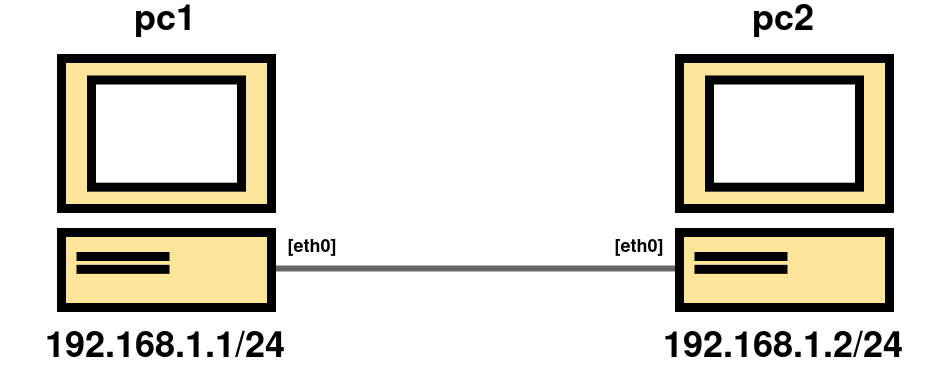
\includegraphics[width=0.8\linewidth]{Images/esempi/lab01.png}
    \caption{Primo scenario.}
\end{figure}

Sono presenti due nodi host, \textbf{pc1} e \textbf{pc2}, il cui traffico è limitato in entrambi secondo questi parametri:
\begin{itemize}
  \item \textbf{Rate:} 1 Mbit$/s$.
  \item \textbf{Burst:} 10 KB.
  \item \textbf{Latency:} 50 ms.
\end{itemize}

\subsection{Soluzione}
In questo primo esercizio, verrà mostrata pure la configurazione per Kathará. Nei prossimi non sarà presente, dato che sarebbe stata molto simile e quindi una ripetizione inutile.
Nello specifico, il primo file è \texttt{lab.conf}, in cui si definisce la struttura principale della rete.
\begin{kathara}[lab.conf]
# Nodo pc1
pc1[0]="A"
pc1[image]="kathara/damper"

# Nodo pc2
pc2[0]="A"
pc2[image]="kathara/damper"
\end{kathara}
Ovviamente, l'immagine usata per i due nodi sarà quella personalizzata con Damper. \\ 
I due host pc1 e pc2 a loro volta dovranno avere il loro file di startup, che segue questo modello:
\begin{kathara}[Modello base per file .startup]
#<host>.startup
ip addr add 192.168.1.x/24 dev eth0
ip link set eth0 up
\end{kathara}
Una volta avviata la rete con il comando \texttt{kathara lstart}, sarà possibile configurare il traffic shaping in user space.
Per prima cosa, dato che non sono presenti vincoli, si deve intercettare tutto il traffico nella tabella OUTPUT per inserirlo in una NFQUEUE nel kernel:
\newpage
\begin{bash}[Regola iptables]
iptables -t raw -A OUTPUT -j NFQUEUE --queue-num 0 --queue-bypass
\end{bash}
Successivamente, andranno modificati i parametri nel file \texttt{damper.conf}, per rispettare le specifiche richieste nello scenario:
\begin{damper}[damper.conf]
# nfqueue queue id
queue 0

# traffic limit in bits per second (suffixes K and M allowed)
limit 1M

# queue length
packets 7
\end{damper}
Così facendo, il rate è limitato a 1Mbit$/s$ e il burst di 10 KB, usando un MTU di 1500 byte, corrisponde a circa 7 pacchetti. Con questi valori si hanno circa 50 ms di latenza. \\
\vspace*{0.01\textheight}
Infine, serve avviare Damper con il comando: \texttt{damper /etc/damper/damper.conf}.

\subsection{Risultati}
\label{sec:res}
Per verificare il funzionamento, si può provare a trasferire un file da un host all'altro, come esempio possiamo scegliere di valutare i tempi da pc1 a pc2.
Per far ciò, è necessario creare un file da poter spedire nel nodo pc1:
\begin{bash}[File da spedire da 1MB]
dd if=/dev/urandom of=file.bin bs=1M count=1
\end{bash}
Successivamente, si mette il nodo pc2 in ascolto con il comando:
\begin{bash}[Comando Netcat]
nc -l -p 8080 > /dev/null
\end{bash}
Infine, si invia il file dal nodo pc1, monitorando il tempo richiesto:
\begin{bash}[Invio di file.bin]
time sh -c "cat file.bin | nc 192.168.1.2 8080 -q1"
\end{bash}
Si può notare che il file, per essere spedito dall'host pc1 all'host pc2, ha impiegato 10 secondi, rispettando quindi il rate di 1Mbit$/s$. \\ 
Il tempo ideali di trasferimento, facendo riferimento alla formula nel capitolo \ref{cap:tc}, sarebbe:
\[
  t = \frac{\text{dim} \times 8}{\text{rate}} = \frac{1 \text{ MB} \times 8}{1 \text{ Mbit}/s} = 8 s
\]
Un margine di circa 2s rimane del tutto accettabile, visto la complessità aggiunta dal dover lavorare in user space.

\section{Limitazione Differenziata verso più Nodi}
Con il secondo scenario, si vuole dimostrare che con Damper è possibile riproporre un funzionamento simile alla disciplina di coda con classi HTB \ref{sec:htb}. \\
Non sarà, quindi, limtato tutto il traffico in uscita, ma valutando la coppia di nodi che comunica.

\begin{figure}[!htb]
    \centering
    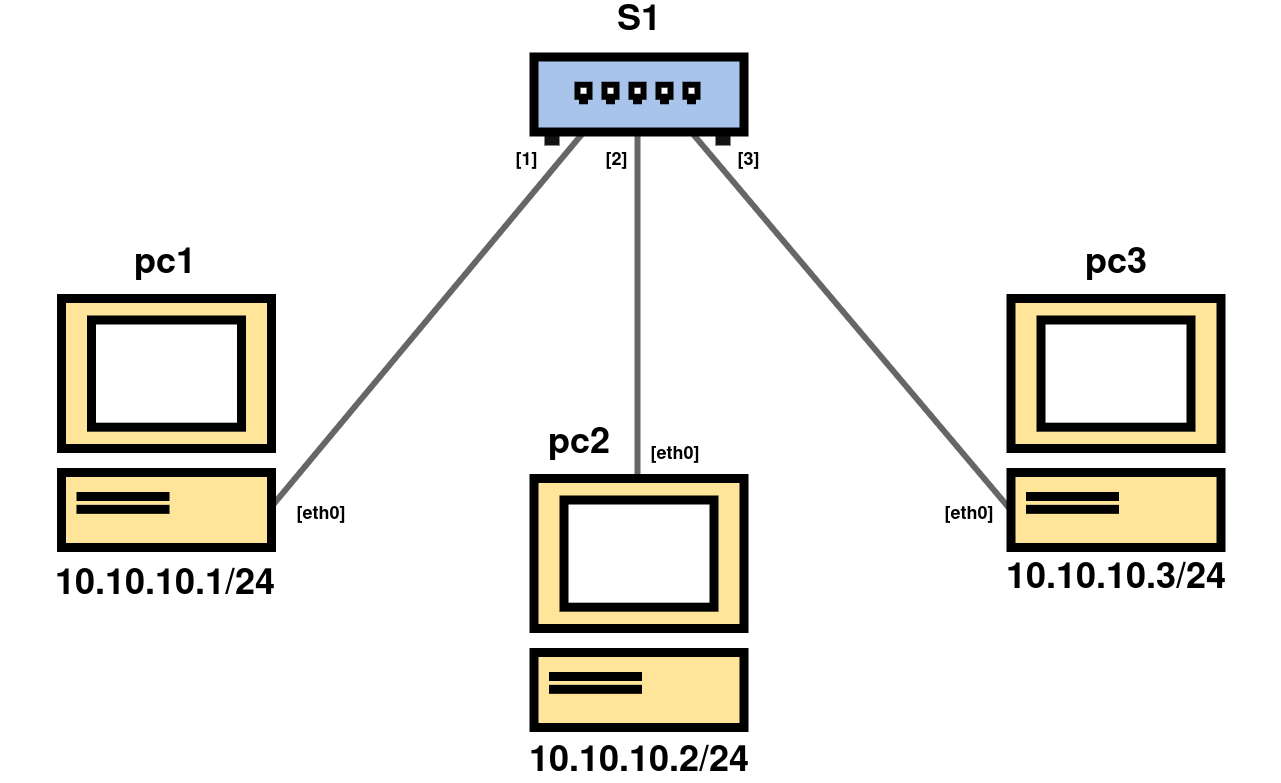
\includegraphics[width=0.8\linewidth]{Images/esempi/lab02.png}
    \caption{Secondo scenario.}
\end{figure}

In questo esempio sono presenti tre nodi: \textbf{pc1}, \textbf{pc2} e \textbf{pc3}, tutti nella stessa rete locale.
Il traffico è diviso in due flussi con velocità diverse:
\begin{enumerate}
  \item \textbf{Slow:} Banda = 1 Mbit$/s$.
  \item \textbf{Fast:} banda $\ge 50 \text{Mbit}/s$ o non limitata.
\end{enumerate}

Ogni coppia di nodi ha diverse combinazioni, per esempio:

\begin{center}
  \begin{tabular}{ |>{\columncolor{gray!35}}c|c|c|c| }
    \hline
    \rowcolor{gray!35}
    $\space$ & \textbf{pc1} & \textbf{pc2} & \textbf{pc3} \\
    \hline
    \textbf{pc1} & $\space$ & slow & slow \\
    \hline
    \textbf{pc2} & slow & $\space$ & fast \\
    \hline
    \textbf{pc3} & slow & fast & $\space$ \\
    \hline
  \end{tabular}
\end{center}

\subsection{Soluzione}
In questo caso, se prendiamo come riferimento l'host pc1, dovrà limitare il traffico sia verso pc2 che verso pc3.\\ 
Damper, però, non simula il comportamento di htb e non supporta nemmeno la definizioni di classi, quindi per farlo funzionare in questo esercizio, 
sarà necessario creare due processi diversi, ognuno con il proprio file di configurazione.
\vspace*{0.01\textheight}
I due file avranno i seguenti parametri:
\begin{damper}[/etc/damper/damper-pc2.conf]
# nfqueue queue id
queue 0

# traffic limit in bits per second (suffixes K and M allowed)
limit 1M

# queue length
packets 7
\end{damper}

\newpage
\begin{damper}[/etc/damper/damper-pc3.conf]
# nfqueue queue id
queue 1

# traffic limit in bits per second (suffixes K and M allowed)
limit 1M

# queue length
packets 7
\end{damper}
Inoltre, il traffico dovrà essere inserito in due NFQUEUE diverse, necessitando di due diverse regole con \texttt{iptable}, dove viene specificato l'ip di destinazione e l'id della coda:
\begin{bash}[Regola traffico verso pc2]
iptables -t raw -A OUTPUT -d 10.10.10.2 -j NFQUEUE --queue-num 0 --queue-bypass
\end{bash}
\begin{bash}[Regola traffico verso pc3]
iptables -t raw -A OUTPUT -d 10.10.10.3 -j NFQUEUE --queue-num 1 --queue-bypass
\end{bash}

Osservando questo esempio, si può notare che i due flussi hanno lo stesso valore di rate, portando a pensare di poter usare lo stesso file e la stessa istanza di Damper per entrambi. \\
Questa soluzione, però, è errata e la risposta si trova nel funzionamento del programma. Se i due flussi condividessero lo stesso processo,
i loro pacchetti sarebbero inseriti nella stassa NFQUEUE in kernel space e nello stesso array in userspace, creando due principali problemi:
\begin{enumerate}
  \item Se le priorità dei pacchetti del primo flusso fossero più elevate rispetto a quelle del secondo e nel caso l'array si riempisse, i pacchetti del secondo flusso verrebbero scartati in favore di quelli del primo.
  \item Il valore di 1 Mbit$/s$ non sarebbe garantito a entrambi, ma sarebbe diviso fra i due flussi.
\end{enumerate}
Per finire e valutare i risultati, devono essere avviate le due istanze del programma:
\begin{bash}
damper /etc/damper/damper-pc2 &
damper /etc/damper/damper-pc3 &
\end{bash}

\subsection{Risultati}
Per valutare le prestazioni si possono ripetere le modalità della sezione precedente \ref{sec:res}, tenendo in considerazione entrambi i flussi verso i rispettivi host. \\ 
Inizialmente, dovranno essere messi in ascolto i due nodi pc1 e pc2:
\begin{bash}[Server nc]
# pc2 
nc -l -p 8080 > /dev/null

# pc3
nc -l -p 8080 > /dev/null
\end{bash}
Per poter calcolare il tempo impiegato dal nodo pc1 per inviare a entrambi il \texttt{file.bin}, creato in modo uguale alla sezione \ref{sec:res}.

\begin{bash}[Nodo pc1]
time sh -c "cat file.bin | nc 10.10.10.2 8080 -q1" & time sh -c "cat file.bin | nc 10.10.10.3 8081 -q1" &
\end{bash}

\begin{bash}[Risultato]
real	0m10.054s
user	0m0.003s
sys	 0m0.007s

real	0m10.151s
user	0m0.003s
sys	 0m0.007s
\end{bash}
Il tempo di entrambi i flussi, 10 secondi ciascuno, è uguale a quello ottenuto nella sezione \ref{sec:res}, rimanendo quindi fedeli al tempo ideale. \\
Inoltre, grazie a questo scenario, si è messo un luce un limite su htb (e in parte tbf) di questo programma in user space. Sarà la principale motivazione del lavoro fatto nel capitolo \ref{cap:donper}.

\section{Limitazione Banda con Gateway/Router}
Quest'ultimo esempoi presenta una scenario diverso rispetto agli altri. Si vuole limitare il traffico verso un host della rete da una sorgente di cui non si ha controllo, 
quindi su cui non si può applicare il traffci shaping con Damper. \\ 
Nella realtà, è una situazione molto comune e di solito viene gestita attravero router o gateway.

\begin{figure}[!htb]
    \centering
    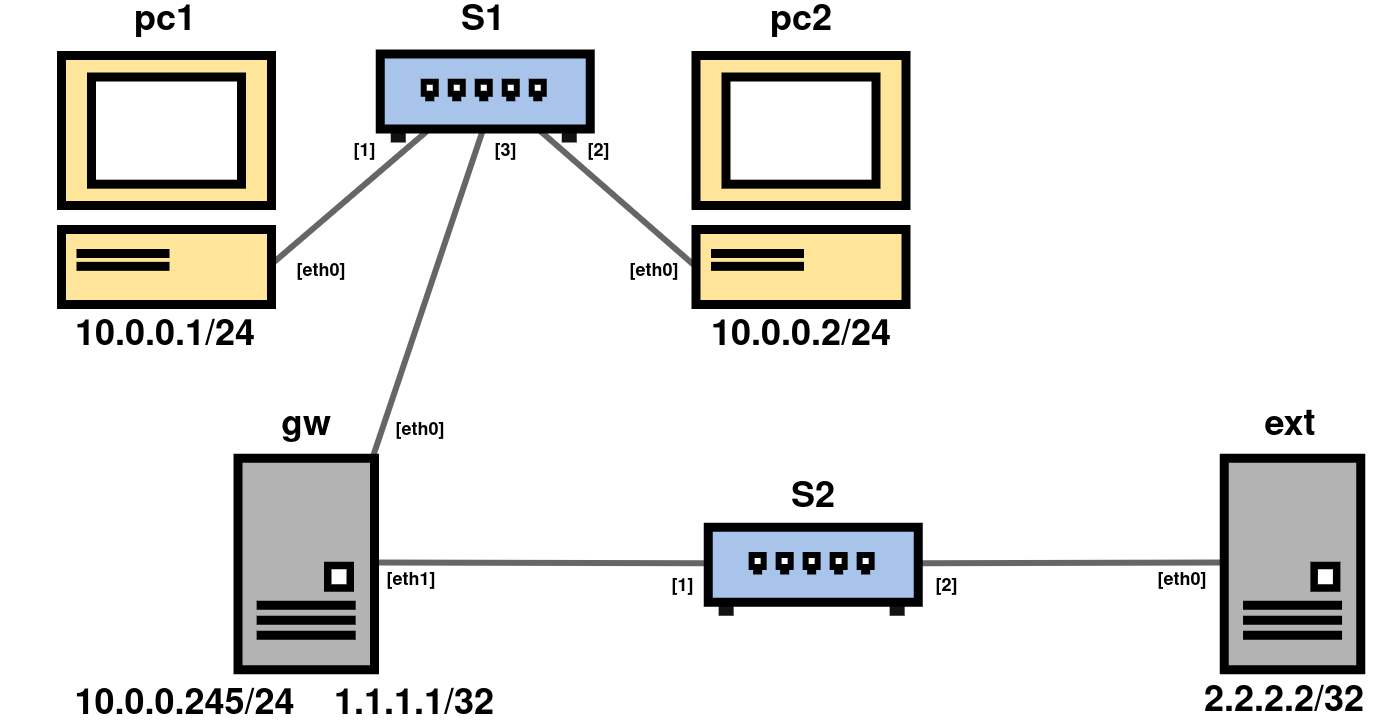
\includegraphics[width=0.8\linewidth]{Images/esempi/lab03.png}
    \caption{Terzo scenario.}
\end{figure}

Nelle rete locale sono presenti due host: \textbf{pc1} e \textbf{pc2} e un gateway \textbf{gw}, che si occuperà del traffic shaping. 
Quest'ultimo, dovra pure permettere il routing fra i nodi della LAN con il server esterno e viceversa. \\ 
\vspace*{0.01\textheight}
Si vuole limitare la banda di pc1 per operazioni di download, per comodità i parametri saranno gli stessi degli esempi precedenti:
\begin{itemize}
  \item \textbf{Rate:} 1 Mbit$/s$.
  \item \textbf{Burst:} 10 KB.
  \item \textbf{Latency:} 50 ms.
\end{itemize}

\subsection{Soluzione}
Come specificato nell'introduzione, lo shaping verrà effettuato dal nodo gw. \\ 
Per iniziare, è necessario scrivare la regola con \texttt{iptables}, per intercettare tutto il traffico verso pc1, assegnandolo alla NFQUEUE numero 0:
\begin{bash}[Regola iptables]
iptables -t raw -A FORWARD -d 10.0.0.1 -j NFQUEUE --queue-num 0 --queue-bypass
\end{bash}
In questo caso, non viene più usata la tabella OUTPUT, ma la tabella FORWARD, visto che i pacchetti non sono generati da un processo dell'host gw, ma da uno del server ext.
\vspace*{0.01\textheight}
Successivamente, come già visto più volte, va configurato il file \texttt{damper.conf} con i parametri giusti:
\begin{damper}[damper.conf]
# nfqueue queue id
queue 0

# traffic limit in bits per second (suffixes K and M allowed)
limit 1M

# queue length
packets 7
\end{damper}
Infine, avviandolo, sarà possibile valutare i risultati.
\begin{bash}[Istanza damper]
damper /etc/damper/damper.conf
\end{bash}

\subsection{Risultati}
Anche in questo scenario, verranno valutati i tempi di invio del file a pc1 tramite gw, paragonandolo, per complettezza, al tempo ideale a 1 Mbit$/s$ e al tempo di invio verso pc2.
Nello specifico, dovranno essere messi in ascolto entrambi i client della rete locale:
\begin{bash}[Server nc]
# pc1
nc -l -p 8080 > /dev/null

# pc2
nc -l -p 8080 > /dev/null
\end{bash}
E dal server ext, di cui in uno scenario reale non si ha controllo, inviamo \texttt{file.bin}, di dimensione 1 MB, verso gli host:
\begin{bash}[Invio file.bin verso pc1 e pc2]
time sh -c "cat file.bin | nc 10.0.0.1 8080 -q1" & time sh -c "cat file.bin | nc 10.0.0.2 8081 -q1" &
\end{bash}

\begin{bash}[Risultato]
real	0m1.201s
user	0m0.002s
sys	 0m0.019s

real	0m10.802s
user	0m0.213s
sys	 0m0.607s
\end{bash}
I tempi rispecchiano i risultati previsti, notando che verso pc1 siano stati impiegati 10 secondi e invece, verso pc2 sia stato impiegato un decimo del tempo.

\section{Limiti di Damper}
\label{sec:limiti}
Nonostante Damper permetta di realizzare il traffic shaping in user space attraverso NFQUEUE,
la sua architettura presenta alcune limitazioni quando si vuole gestire contemporaneamente traffico appartenente a classi diverse.
Nello specifico, lo shaping è basato su un'unico vettore di pacchetti e su un unico limite di banda associato al processo in esecuzione. \\ 
\vspace*{0.01\textheight}
Nel capitolo successivo, spiego il motivo che mi ha portato allo sviluppo di \textbf{Donper} \cite{donper}, un fork di Damper nel quale ho introdotto una struttura gerarchica per la gestione dei pacchetti, 
implementando un l'algoritmo di prestito e la divisione in classi. 
Con questa modifica, è stata aggiunta una gestione dei pacchetti di Damper simile a discipline di accodamento come tbf e htb.
